\documentclass[12pt]{article}
\usepackage[utf8]{inputenc}
\DeclareUnicodeCharacter{2212}{-}

%STYLE
\usepackage{helvet} %HELVETICA
\usepackage{dirtytalk}
\usepackage{hyperref}
\hypersetup{
    colorlinks=true,
    linkcolor=mygray,
    filecolor=magenta,      
    urlcolor=blue(pigment),
    citecolor=mygray,
}

%\urlstyle{same}

\usepackage[usenames,dvipsnames, table]{xcolor}%remove green borders from links but still make it understand that are cliccable

\definecolor{mygray}{gray}{0.6}
\definecolor{blue(pigment)}{rgb}{0.2, 0.2, 0.6}

%BIBLIOGRAPHY STYLE
\usepackage{natbib}
\bibliographystyle{agsm} %Imperial College Harvard Style
\usepackage{authblk} %Add second authors and affiliations
\renewcommand{\bibsection}{} %Hide 'References' header

%FIGURE OPTIONS
\usepackage{float} %position images
\floatstyle{plaintop}%Caption on top of tables
\restylefloat{table}
\usepackage{graphicx, caption}
\graphicspath{ {./images/} }
\usepackage{mathtools}
\usepackage{amsmath}
\usepackage{stackrel,amssymb}
\usepackage[inline]{enumitem}
%\captionsetup{font= doublespacing}
\captionsetup{width= 6.5in}


%GEOMETRY
\usepackage[left=2.3cm,right=2.3cm,top=2cm,bottom=2cm]{geometry}
\usepackage{setspace}
\doublespacing
\usepackage{multirow}
\setlength{\parindent}{0em}
\usepackage{changepage}

\setlength{\textfloatsep}{0.1cm}


\begin{document}


\begin{Large}
\textbf{Mapping the Nucleotide Sequence of the PrqR Operator of \textit{Synechocystis sp.} PCC 6803 with Reporter Plasmids}
\newline
\end{Large}
Alberto Scarampi
\newline
14/05/2021\\
\noindent\rule{\textwidth}{0.4pt}

\section*{Summary}
In this experiment \textit{E. coli} cells will be transformed with plasmids encoding fluorescent reporter proteins downstream of synthetic promoters to investigate whether the PrqR transcription factor displays ``in-trans" repression activity via a putative operator sequence found in the promoter region of the prqRA operon of \textit{Synechocystis sp.} PCC 6803.

\section*{Introduction}
In the model cyanobacterium \textit{Synechocystis sp.} PCC 6803, a spontaneous mutant (prq20) was previously shown to be resistant to externally added methyl viologen (a photosynthetic inhibitor commonly sold as a herbicide under the name of Paraquat) \citep{Kirik2003}. 
In this strain, the prqR gene was found to encode a missense mutation (L17Q) in in the N-terminal DNA-binding domain of PrqR, which resulted in derepression of the prqR–prqA operon, where prqA codes for a predicted transmembrane antiporter protein.
Additionally, \cite{Kreslavski2007} observed that the photosynthetic apparatus was less affected in the prq20 mutant than in the wild type (WT), as indicated by the damage generated by two strong-oxidative-stress producing compounds (methyl and benzyl viologen).
More recently, \cite {Khan2016} reported that the deletion mutant ($\Delta$prqR) showed increased growth rate and decreased reactive oxygen species (ROS) content, whereas the complementary strain (CprqR) restored the growth characteristics, phenotypes and ROS status of WT, thereby establishing PrqR as a negative regulator of ROS. Further study by qRT-PCR, ChIP-PCR and deletion of both prqR and prqA revealed that PrqR exerts this negative regulation of ROS removal by controlling the expression of sodB and prqA (slr0896). Furthermore, PrqR also found to control glucose metabolism by regulating a positive regulator of glucose metabolism, sigE, and its regulons.
Taken together, these results confirm that PrqR is a transcription factor with the ability of repressing itself and other genes involved in sensing and adaptation to oxidative stress. However, there are many aspects still unknown about the regulation exerted by this redox-sensitive transcription factor.
In particular, it is unclear how PrqR is able repress itself and what inhibits this autorepression (i.e. what induces expression of PrqR).
By expressing PrqR (together with its 5' upstream DNA sequence) in \textit{E. coli}, \cite{Kirik2003} already suggested that prqR may be auto regulated via PrqR binding to operator sites in the promoter region. Their experiment was conducted by fusing the prqR gene (together with its 5' upstream sequence) to the cat gene (conferring chloramphenicol resistance) and repression activity was quantified by measuring cell growth inhibition in the presence of chloramphenicol. However, the upstream promoter region they cloned upstream of prqR was very long (more than 1000 bp including also part of the gene upstream of prqR) it is hard to map where exactly this operator region is. In addition, the use of cell growth inhibition at steady state as a measure for transcriptional activity of PrqR is limiting as it fails to capture the full expression and cannot be used to estimate parameters (e.g. maximal and inhibited transcription rate) that would be useful to model the genetic expression of this interesting redox-dependent transcription factor.
For this reasons, an experiment is here proposed that aims to address these limitations using more up-to-date techniques (shorter and rationally designed upstream sequence using GoldenGate DNA assembly and no antibiotic resistance gene but fluorescent protein as reporter). 

\section*{Research Questions}
\begin{itemize}
    \item Does the PprqR promoter encode an operator region responsible for direct interaction with the PrqR repressor?
    \item If yes, what is the nucleotide sequence of such region ?
\end{itemize}

\section*{Experimental Design}
In order to address the questions above, this experiment proposes to construct and measure the fluorescence of reporter plasmids containing strong constitutive \textit{E. coli} promoters mutated to encode putative PprqR operator sequences. These plasmids will also contain the prqR coding sequence under the control of the inducible lac promoter, in order to quantify the potential repression activity exerted by the PrqR repressor.
Initially, this experiment will be performed in \textit{E. coli} cells for ease of cloning and quantification of fluorescence using a plate reader. If significant repression is observed in in \textit{E. coli} containing the promoter with the putated operator sequence compared to control promoters, this would suggest a direct, ``in-trans" repression activity exerted by the PrqR repressor. This finding would be consistent with the regulation displayed by other members of the TerR-like family of transcription factors. 
On the other hand, if no significant differences in fluorescence are observed, this would suggest that either the operator sequence is found farther than 100 bp upstream of the start site (very unlikely for eubacterial promoters) or that the regulation mediated by PrqR is dependent on \textit{Synechocystis}-specific factors not present in \textit{E. coli}. In the latter case, this experiment will be repeated by transforming the same plasmids in \textit{Synechocystis} cells.

\subsection*{Analysis of the PprqR Promoter and its Sequence Motifs}
To identify putative operator sequences in the PprqR promoter, this sequence was first identified and annotated in the genome of \textit{Synechocystis sp.} PCC 6803. This was performed by identifying the DNA sequence extending 100 bp upstream of the first A nucleotide in the start codon (ATG) of the prqR gene. As shown in Fig. \ref{fig:motifs}, this sequence was aligned for comparison with other well-characterised  \textit{E.coli} promoters. Using promoter and RBS prediction softwares (\href{http://www.bacpp.bioinfoucs.com/home}{BacPP}, \href{https://salislab.net/software/}{RBS calculator}), it was possible to identify certain features in the promoter sequence, such as the ribosome binding sites (RBS), the core promoter elements. According to \cite{Gordon2018}, cyanobacterial promoters can be categorised into three groups based on their sequences and which sigma factors recognise them. Type I promoters (recognised by $\sigma$70) contain both a −10 element (consensus 5’-TATAAT-3’) and a −35 element (consensus 5’-TTGACA-3’). Type II promoters contain the −10 element but lack a −35 element, instead containing operator sites bound by transcription factors. Type III promoters lack −10 or −35 elements and generally respond to various stresses through binding of type III sigma factors.
$P_{prqR}$ might be a type II promoter. In fact it contains a −10 element but the sequence at the −35 location is quite dissimilar to the -35 consensus (5’-TTGACA-3’), and instead contains an upstream sequence with two heptameric repeats and two palindromes, which might encode the operator region.

\begin{figure}[H]
    \centering
    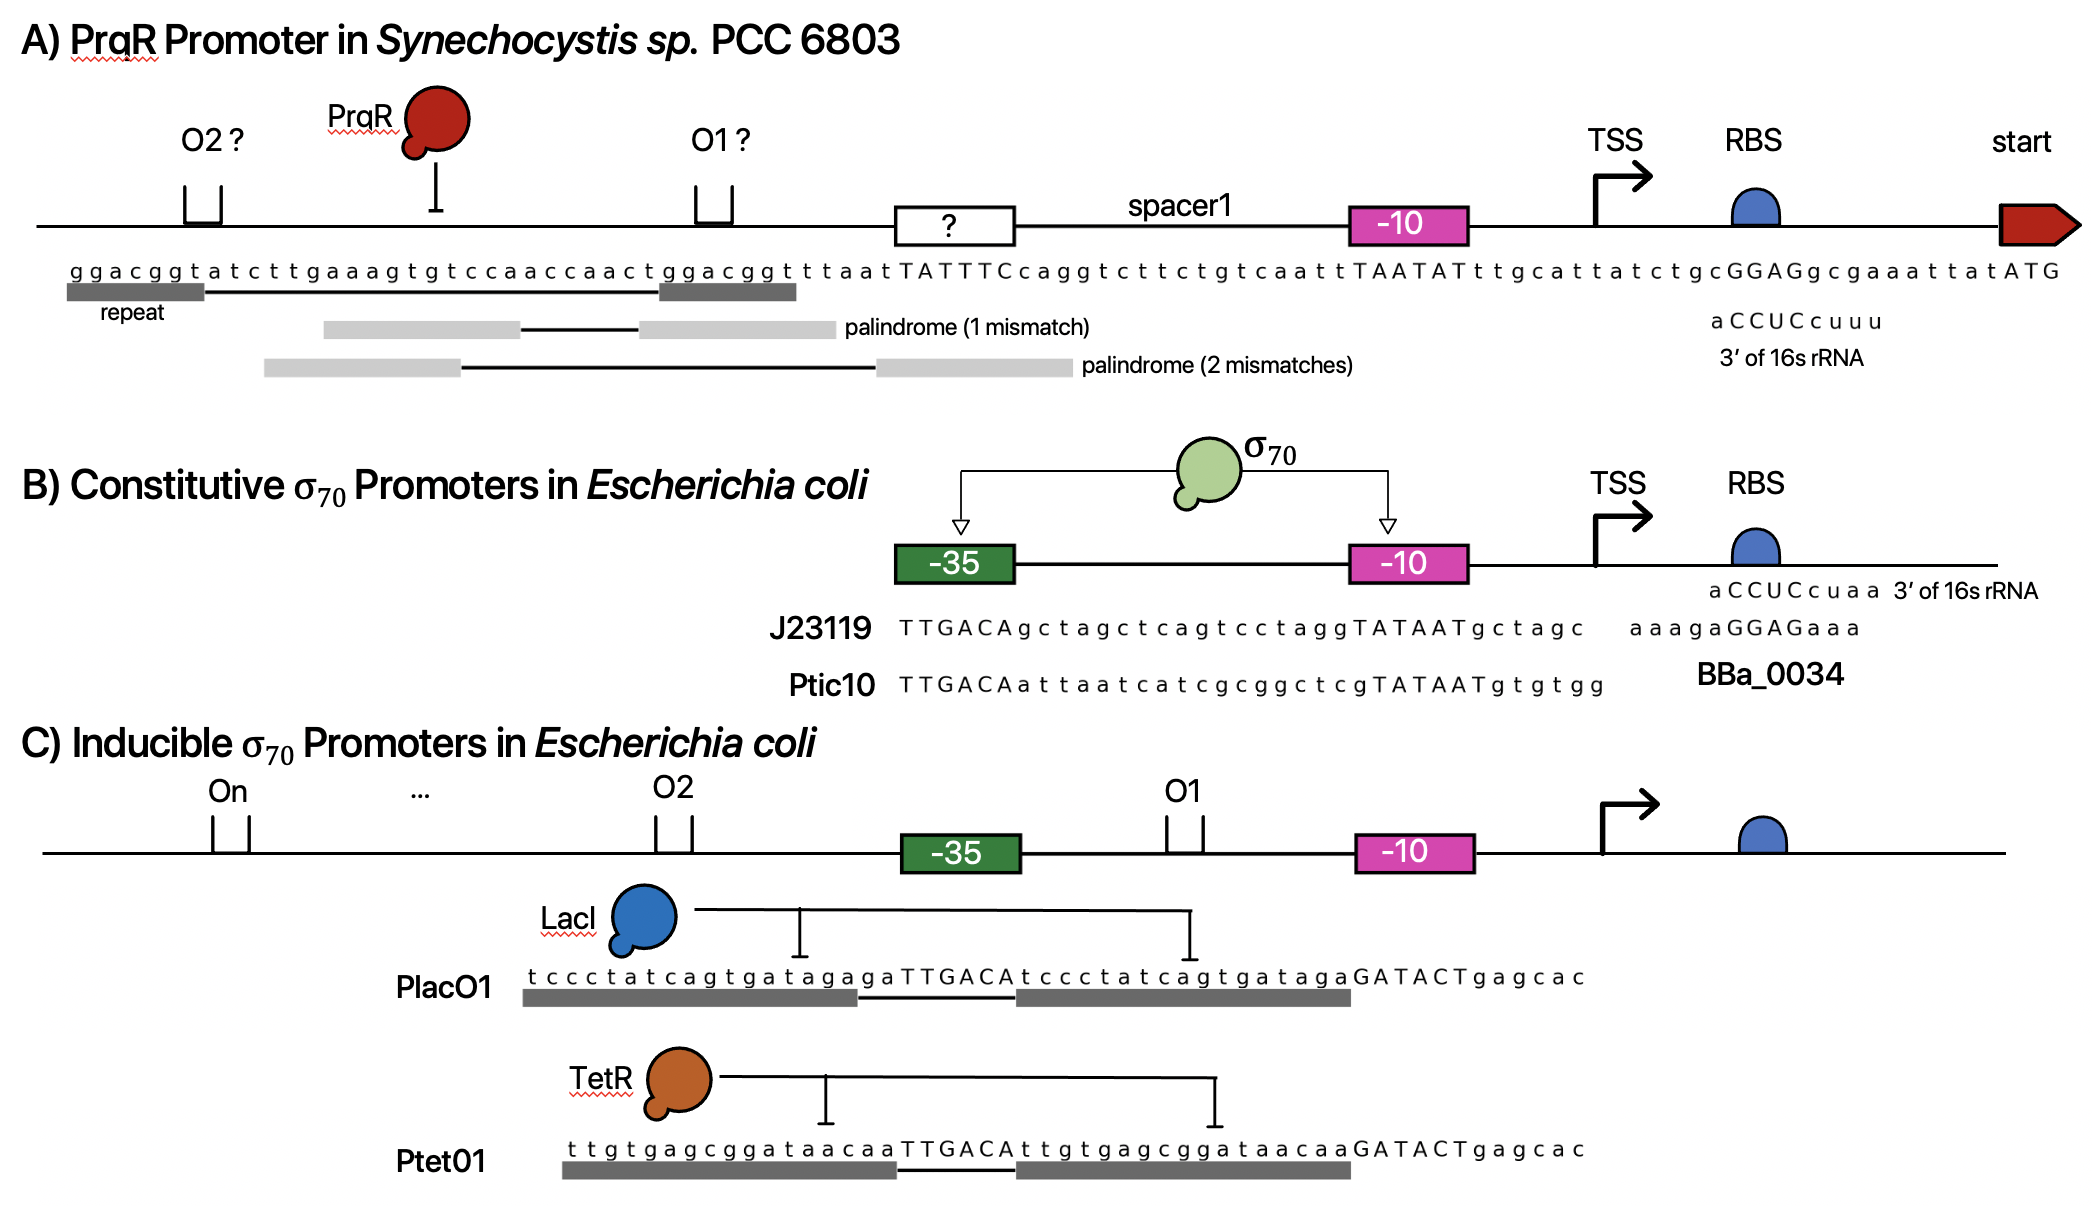
\includegraphics[width=\textwidth]{images/f1reporters.png}
    \caption{Comparison between the PrqR promoter under study and representative $\sigma_{70}$ promoters in \textit{E. coli}. The green and purple boxes represent core promoter elements recognised by $\sigma_{70}$ factor. It is unknown what $\sigma$ factor recognise the PrqR promoter in \textit{Synechocystis}.On the other hand, in growing \textit{E. coli} cells, most promoters are regulated by $\sigma$70, a housekeeping transcription factor that bind conserved hexameric sequences within a promoter sequence and enables RNA polymerase to initiate transcription \citep{Chen2018}. This class of promoters is the most well-characterised and its member display highest constitutive expression.}
    \label{fig:f1}
\end{figure}

Interestingly, the analysis shown in Fig.\ref{fig:f1} revealed that the region upstream of the core promoter elements in the PrqR promoter harbours a repeated heptameric sequence in close proximity to palindromic sequences. Given that repressors of the TetR-like family often bind DNA as oligomers, this sequence seems to be an ideal candidate for an operator region. 
Given that each sequence position could encode 4 possible nucleotides (A, C, G, T), the probability of finding this specific heptameric sequence by chance would be $4^{7} =$ 1 every 16384 bp. However, in this specific promoter region (42 bp) two of these exact heptameric sequences are repated, which is significantly more than expected by chance. This conservation of nucleotide sequence might suggest biological relevance.

Additional bioinformatic evidence further suggest why conserved repeat . As a transcription factor that regulates response to oxidative stress, it is likely that PrqR might exert its repressor activity to regulate other genes. If this regulatory mechanism is mediated ``in-trans" by an operator sequence, a sequence motif recognised by the DNA-binding domain of PrqR is expected to be found upstream of the gene regulated by the PrqR.
For this reason, the repeated sequence motif GGACGGTN(10,20)GGACGGT (heptameric sequence separated by any spacer region between 10 ans 20 bp long, max 2 mismatches allowed) was used as query to perform a blastn search against the genome of \textit{Synechocystis sp.} PCC 6803.
Fig.\ref{fig:motifs} shows the name of the genes whose upstream region (between 100 bp upstream and start codon of gene) display a hit for the motif search described above.
As shown by the regions highlighted in black, this repeated heptameric sequence seems to be conserved in regions upstream of other genes than PrqR. Interestingly some of these upstream motif-containing genes are also implicated in redox metabolism.
\begin{figure}[H]
    \centering
    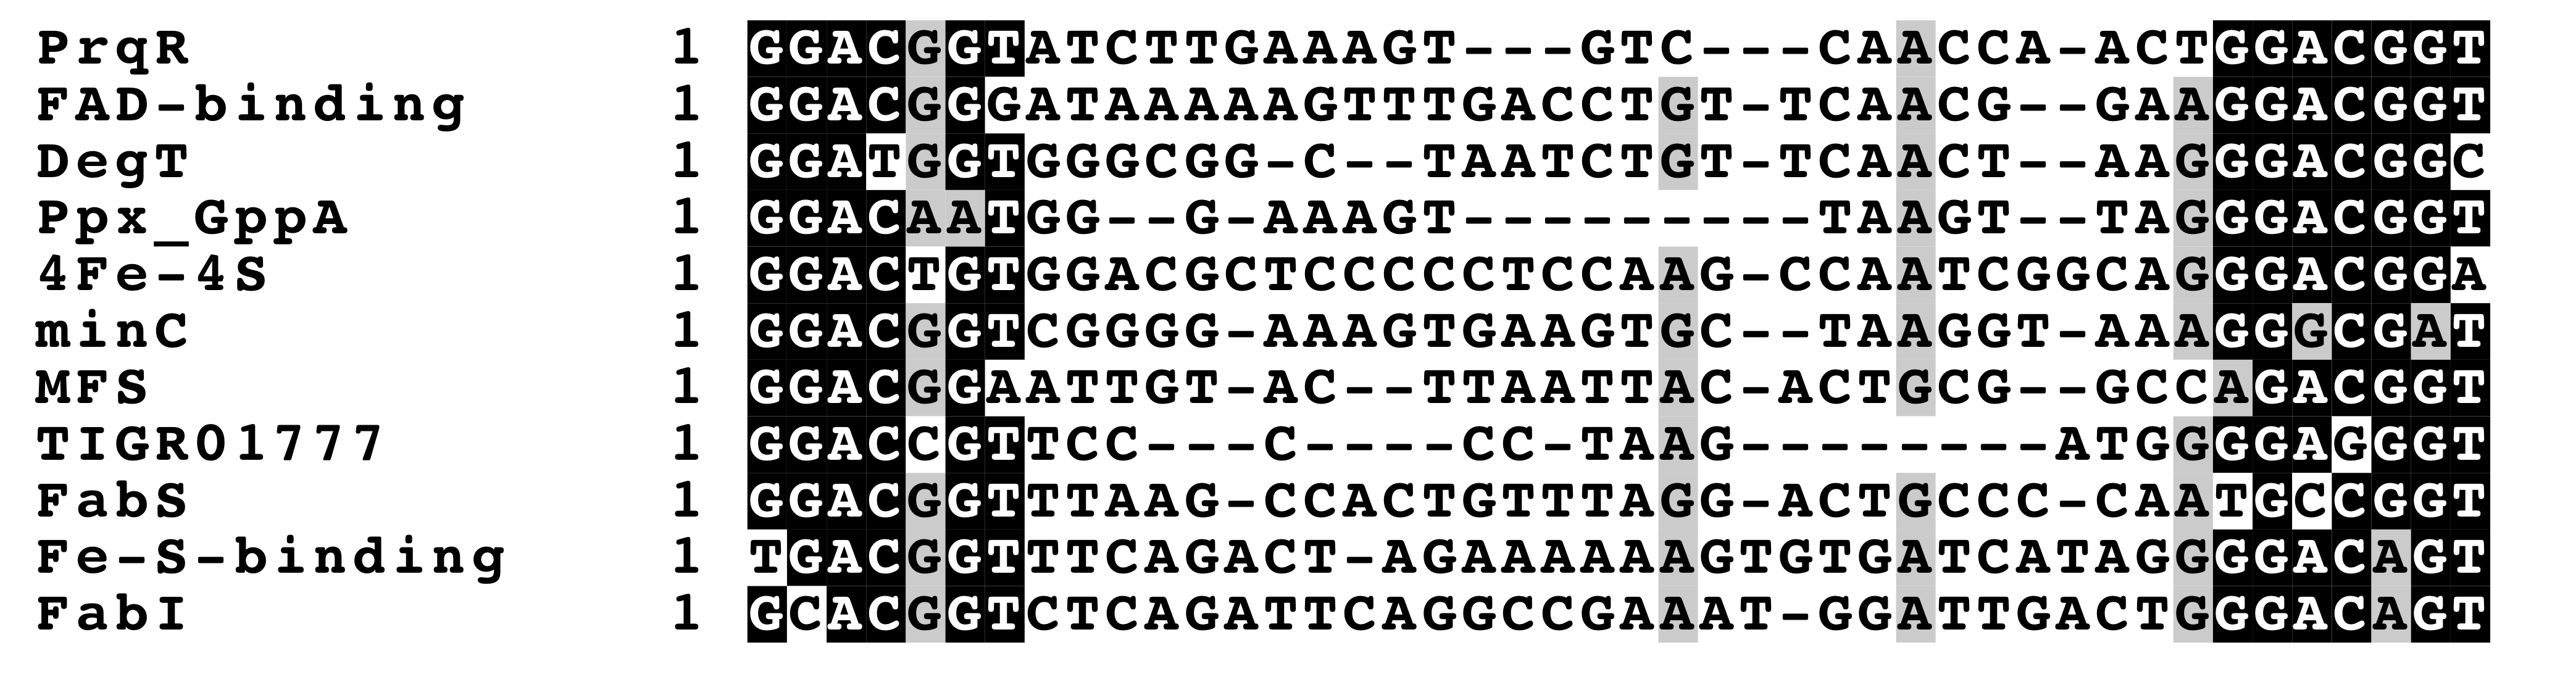
\includegraphics[width=\textwidth]{images/prqR_motif.png}
    \caption{Heptameric nucleotide sequence motifs found upstream of CDS in the genome of \textit{Synechocystis sp.} PCC 6803. Name and locus tag of the genes from top to bottom: prqR (WP\textunderscore010873672.1), FAD-binding oxidoreductase (WP\textunderscore010871487.1), DegT family aminotransferase (WP\textunderscore010874267.1),  Ppx/GppA family phosphatase (WP\textunderscore010874262.1), 4Fe-4S binding protein CDS (4Fe-4S binding protein), minC (WP\textunderscore010873891.1), MFS transporter (WP\textunderscore010873841.1), TIGR01777 family oxidoreductase CDS (WP\textunderscore014407090.1), fabF (WP\textunderscore010871941.1), (Fe-S)-binding protein CDS (WP\textunderscore010871774.1), fabI (WP\textunderscore014407072.1)}
    \label{fig:motifs}
\end{figure}


\subsection*{Promoter Design and DNA Assembly of Reporter Plasmids}
Preliminary experiments have revealed that in \textit{E. coli} expression of eYFP under the native \textit{Synechocystis} PrqR promoter results in fluorescence emission significantly lower than the positive control consensus promoter J23119. This might be because PrqR contains a cyanobacterial RBS and might not be recognised by the \textit{E. coli} $\sigma_{70}$ factor (PrqR has not TTGACA -35 and has TAATAT instead of TATAAT -10). For this reason,  synthetic promoter sequences containing a constant strong \textit{E.coli} RBS ($BBa\textunderscore0034$) and a J23119 scaffold have been designed, as shown in Fig. \ref{fig:promoters}.

\begin{figure}[H]
    \centering
    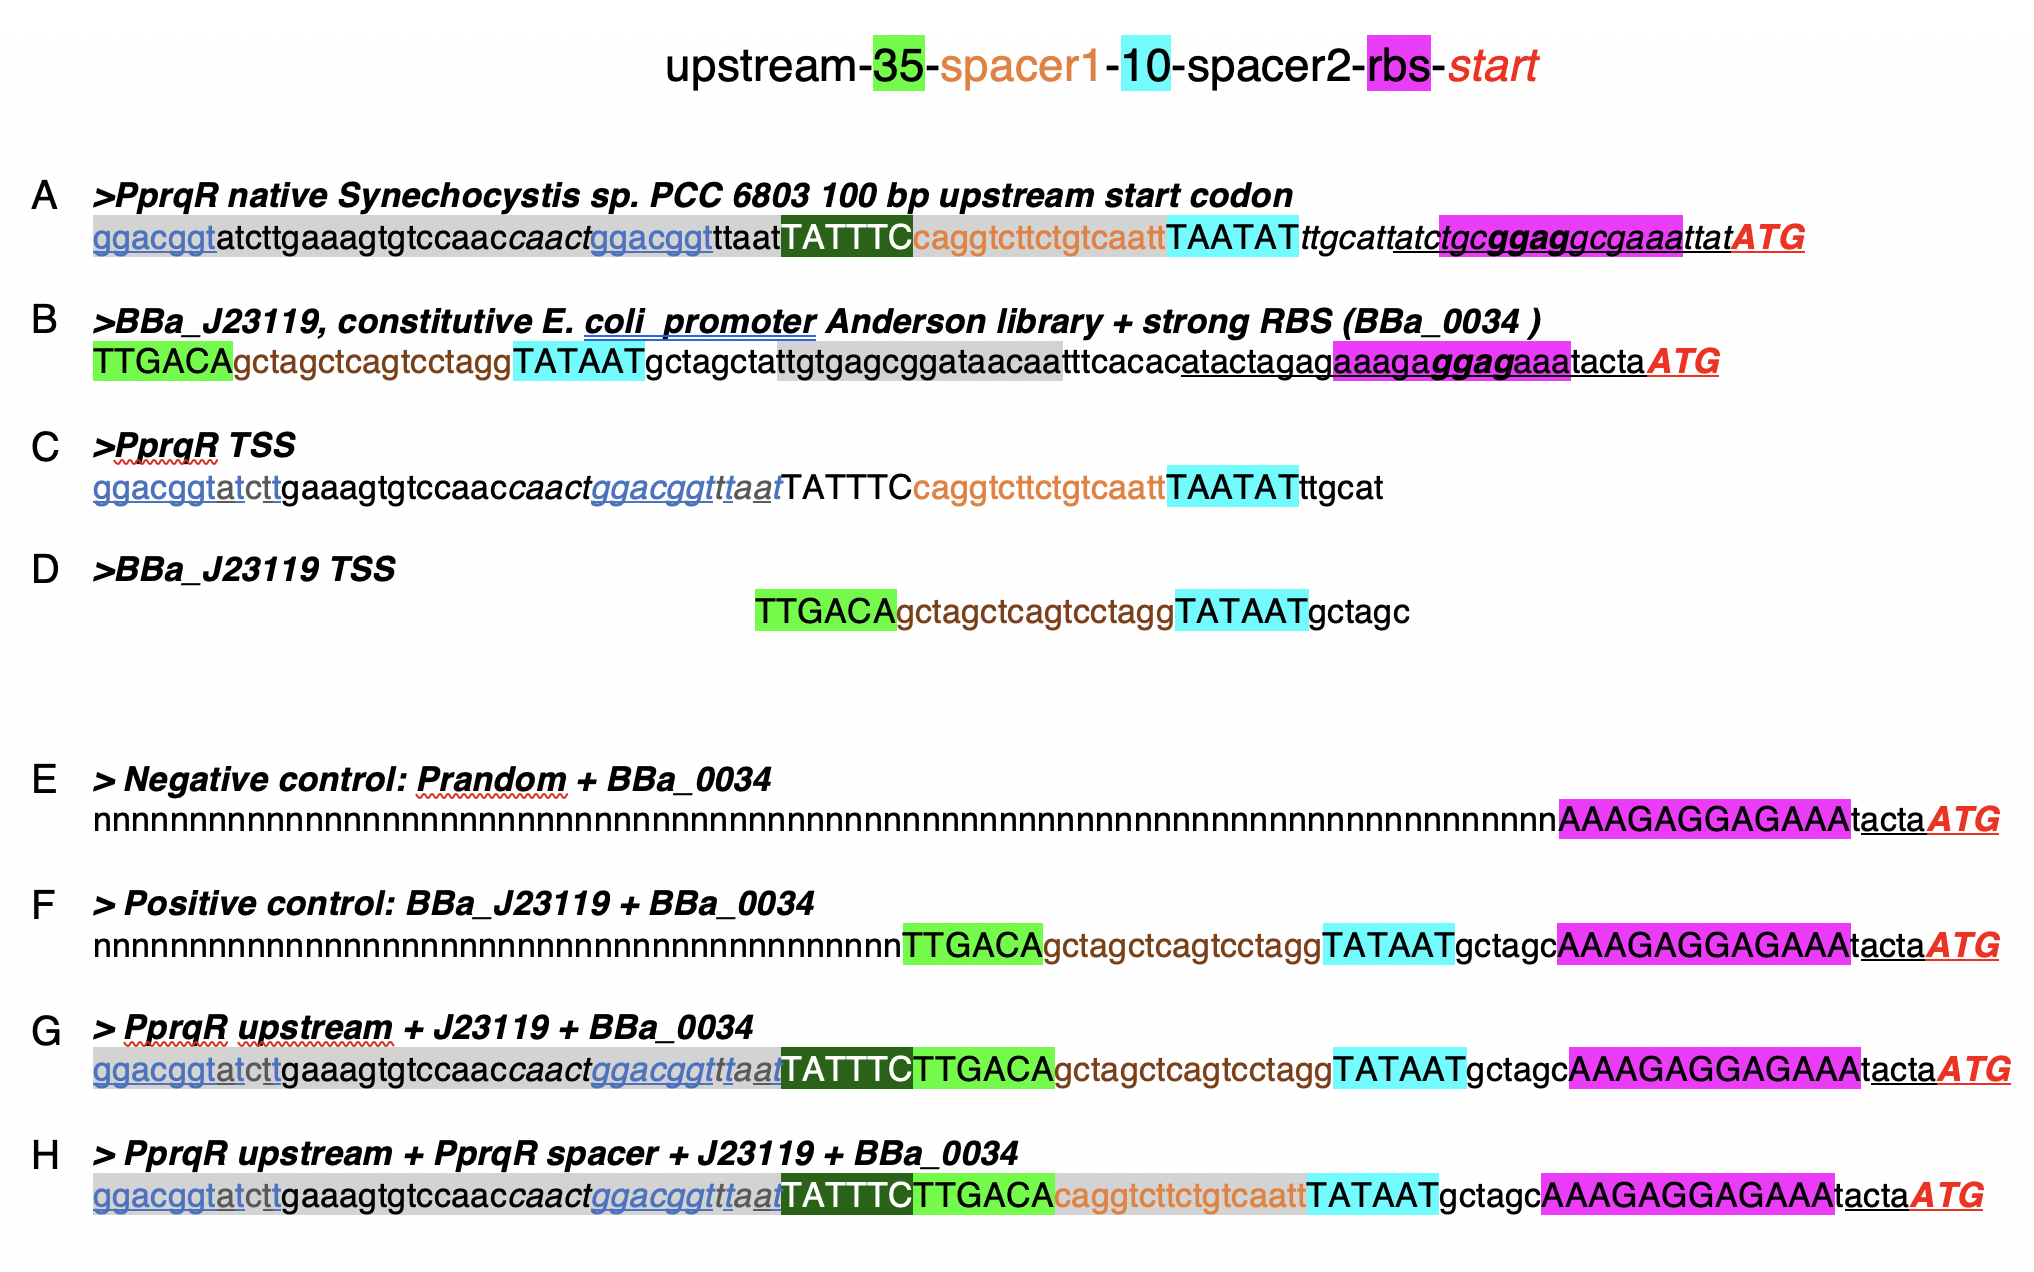
\includegraphics[width=\textwidth]{images/operator_promoters.png}
    \caption{Oligonucleotide sequences (5'$\rightarrow$3') of the synthetic promoters to test the test efffect of putative PrqR operator sequences on the expression of a fluorescent reporter (after ATG). A-B) Sequences of the promoters tested already. C) Truncated versions of PprqR without cyanobacterial RBS (TSS). D) Core promoter elements of consensus promoter (J23119). E-H) The new synthetic promoter sequences that will be used for the experiment here proposed. The sequences will be made all of the same length by the addition of random nucleotides (n). Each of the promoters will be assembled by annealing 4 set of oligonucleotides containing complementary 4 bp overhangs and CyanoGate prefix (GGAG) and suffix (AATG) compatible for assembly into a level 0 promoter acceptor (pICH41276).
These 4 possible promoters will be then cloned upstream of a level 0 CDS eYFP part (pC0.008) and PclpPX terminator (parts already available).}
    \label{fig:promoters}
\end{figure}

\subsection*{Measuring Fluorescence Output from Reporter Plasmids}
All the promoters + eYFP + Terminator constructs will be cloned in a backbone plasmid containing prqR downstream of the IPTG-inducible lactose operator. In this way by measuring the fluorescence emitted by \textit{E. coli} cells transformed with the various promoter types it is possible to quantify the strength of each promoter in the absence  or presence of the repressor PrqR.
\begin{figure}[H]
    \centering
    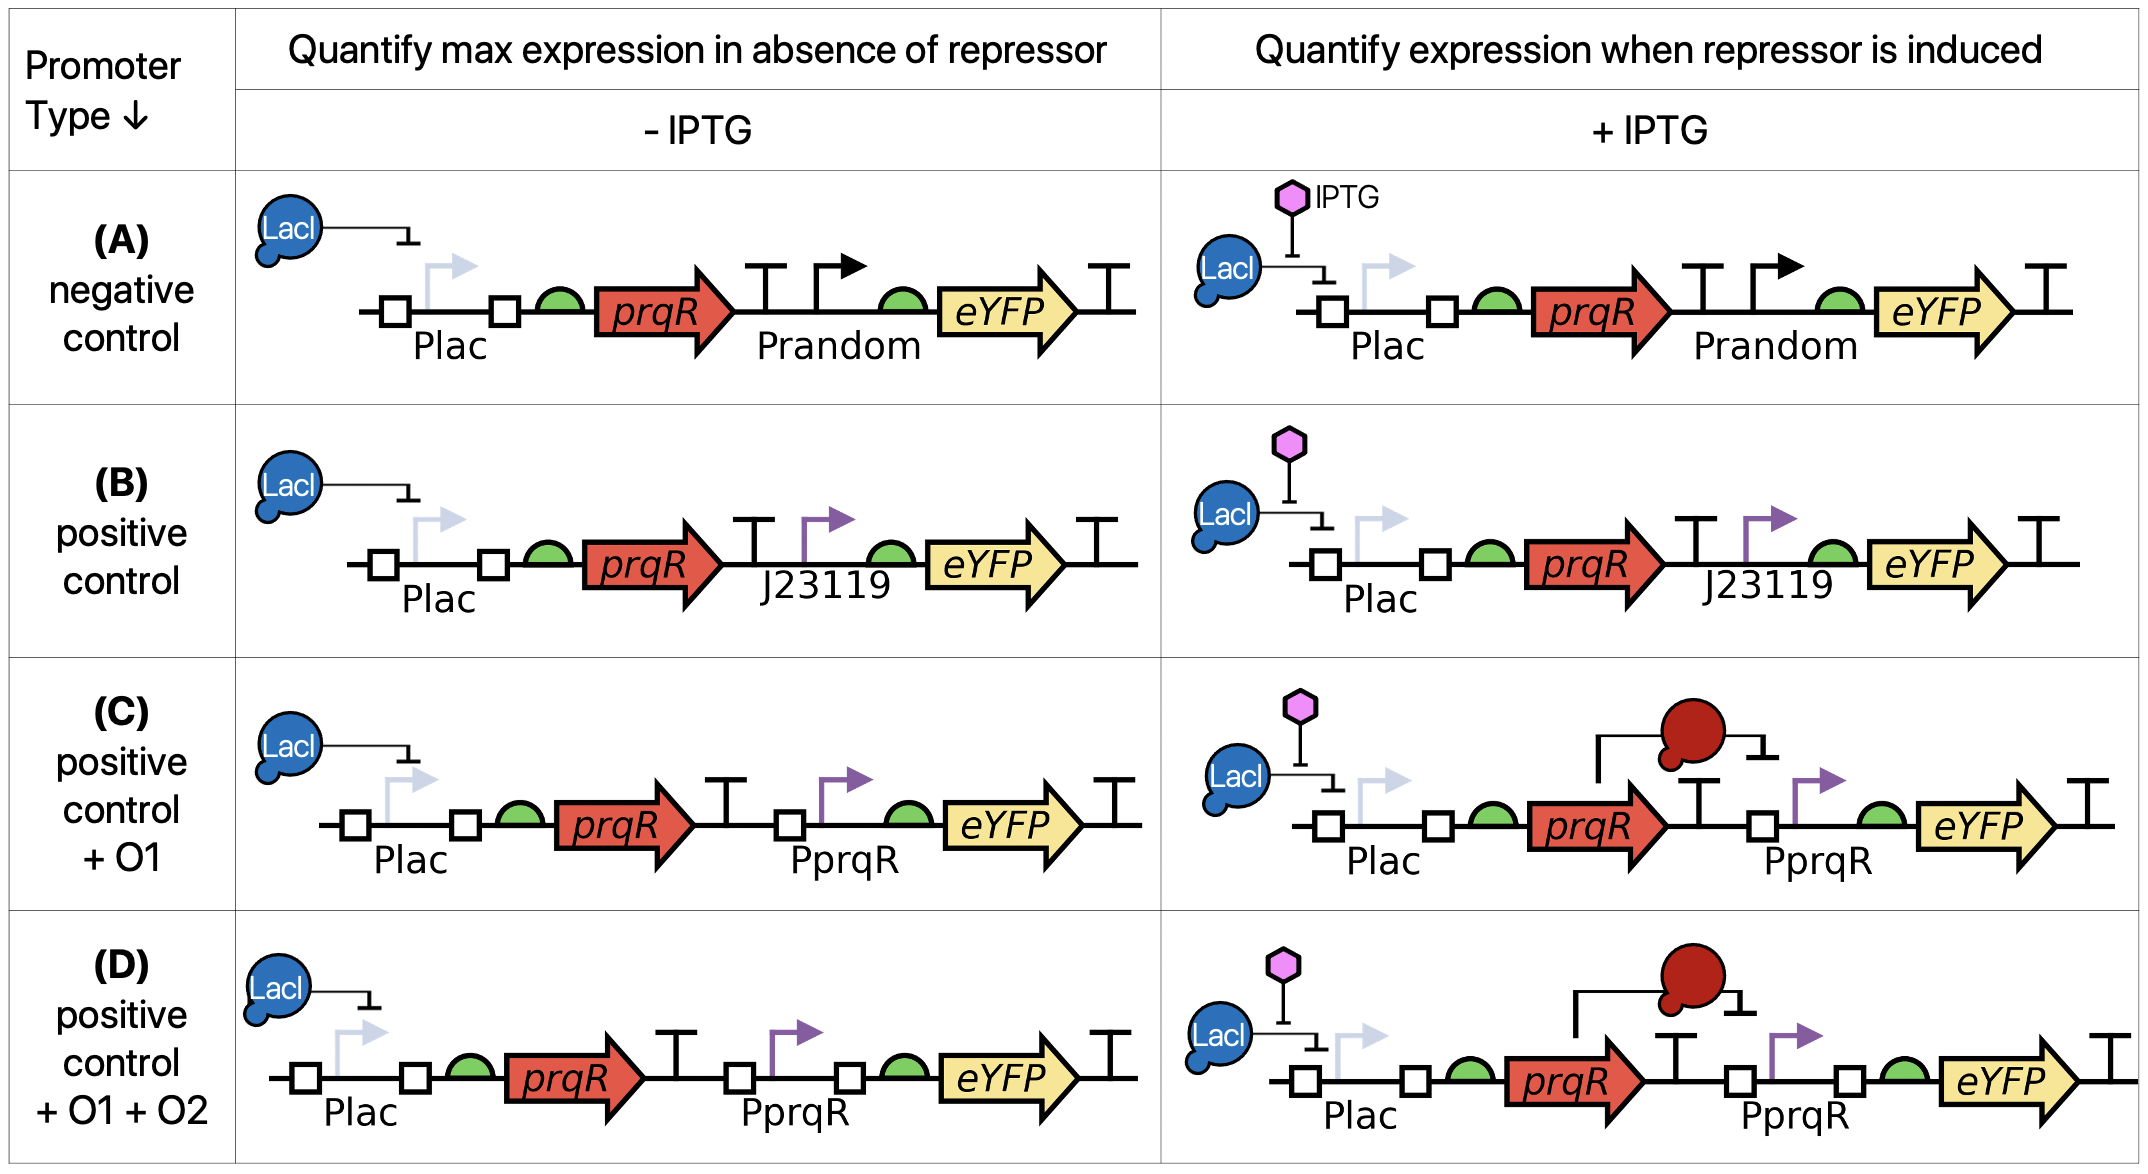
\includegraphics[width=\textwidth]{images/operator_plasmids.png}
    \caption{Reporter plasmids used to quantify the maximal and inhibited expression in the presence of putative operator sequences. Fluorescence profiles from the negative control plasmid can be used to blank background fluorescence of eYFP in \textit{E.coli}. Fluorescence profiles from the positive control plasmid quantify maximal expression expected from J23119 promoter scaffold. Fluorescence profiles from plasmids C and D can be used to estimate the potential repression activity mediated by either operator O1 (upstream element of PrqR) or O2 (upstream + spacer1 from prqR promoter).}
    \label{fig:plasmids}
\end{figure}
If the expression strength for either plasmid C or D in the +IPTG condition is significantly lower than the in -IPTG while the fluorescent profiles of plasmid A and B remained unchanged (min and max fluorescence respectively), this would indicate that the putative operator region of the PrqR promoter is responsible for direct DNA-Protein interactions with the repressor PrqR.

\section*{References}
\bibliography{bibliography.bib}

\end{document}